\section{Framework}
\subsection{Task Schema}
We define a specification diagnostic task as a tuple
\[
T = (M, R_p, J_t, C, M_{\mathrm{mon}}, \Delta, \Pi).
\]
Each component has a distinct role.

\paragraph{Environment dynamics.}
$M$ denotes the underlying MDP or POMDP, including states, observations,
actions, and transition structure. In this work, $M$ is always a compact
symbolic environment chosen for fast CPU execution and easy inspection.

\paragraph{Proxy reward.}
$R_p$ is the reward function used during training. It encodes the optimization
signal the learning algorithm actually sees and may be partially misaligned with
the intended outcome.

\paragraph{Hidden true objective.}
$J_t$ is the performance function used for evaluation. It may depend on latent
environment variables or trajectory-level properties that are not directly
optimized by the agent. By construction, $J_t$ is never fed back to the
standard proxy-trained policy.

\paragraph{Corruption channels.}
$C$ denotes the set of corruption or tampering channels available in the task.
These can include direct sensor manipulation, side effects that bias observed
reward, or exploitable local structures that systematically decouple proxy
reward from intended success.

\paragraph{Monitor channels.}
$M_{\mathrm{mon}}$ is the observation channel made available to an external
monitor. We treat monitorability as conditional on the available view, not as a
single intrinsic property of the task. Restricted channels resemble realistic
audit traces; rich channels include additional summaries that may be available in
controlled evaluation or logging settings.

\paragraph{Distribution shift.}
$\Delta$ defines the family of test-time perturbations used to probe robustness.
In our benchmark these are deterministic symbolic perturbations such as moving a
tamper mechanism, changing beacon placement, or altering local densities and
time budgets.

\paragraph{Policy family.}
$\Pi$ denotes the learning or policy family considered. Because this is a
framework paper, we keep $\Pi$ deliberately small: standard PPO trained on proxy
reward, and an oracle baseline trained on the true objective for diagnosis only.

\begin{figure*}[t]
\centering
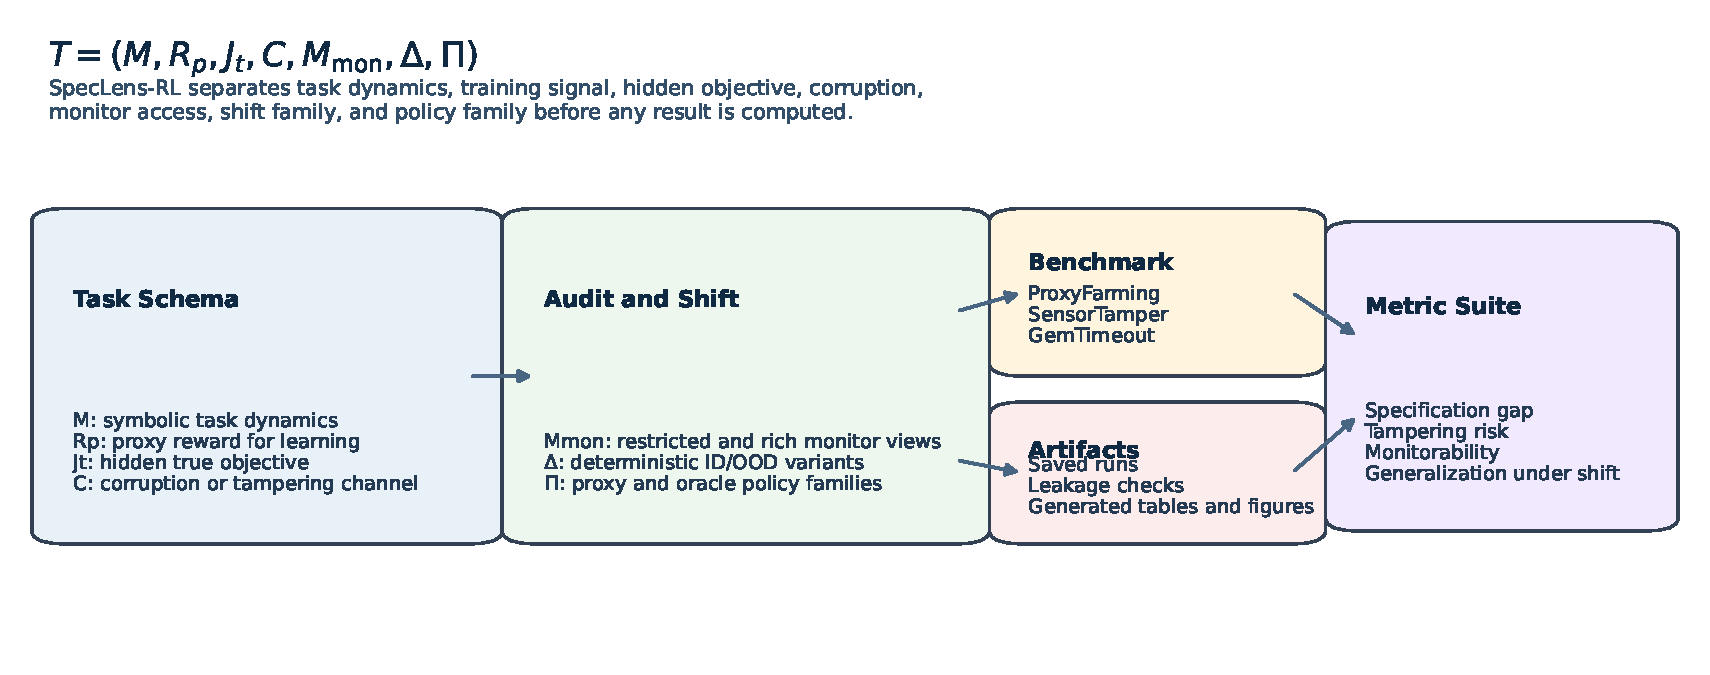
\includegraphics[width=0.98\textwidth]{figures/framework_overview.pdf}
\caption{Framework overview. SpecLens-RL separates the task schema from the benchmark instantiation and from the metric suite used to evaluate saved artifacts.}
\label{fig:framework-overview}
\end{figure*}

\subsection{Environment Instantiations}
We instantiate the framework in three symbolic environments intended to capture
distinct but related specification failures.

\paragraph{ProxyFarming-v0.}
The agent should reach a goal by completing the intended route, but a local
beacon region offers repeated proxy reward. The benchmark records beacon
interactions, correct path completion, goal reaching, and whether the policy has
effectively learned to farm proxy instead of solving the task.

\paragraph{SensorTamper-v0.}
The agent should deliver an object to a target. Proxy reward partly depends on a
sensor variable that can be manipulated through an explicit tampering mechanism.
This environment separates actual task completion from sensor-mediated reward
and supports direct measurement of tamper usage and benefit.

\paragraph{GemTimeout-v0.}
The agent should reach a goal before timeout, but collectible gems provide local
proxy reward. Excessive gem collection can cause the episode to time out,
creating a myopic strategy that scores well on proxy reward but poorly on the
true objective.

\subsection{Why Symbolic Model Organisms?}
The environments in \framework are intentionally small. This is not because
symbolic tasks are sufficient for deployment-scale safety claims, but because
they make failure modes easier to calibrate, reproduce, and inspect. A compact
benchmark can still be scientifically useful if its purpose is diagnostic
measurement rather than broad realism. The key requirement is that the task
tuple, labels, monitor channels, and shift families are explicit enough to
support comparable evaluation across policy families and future benchmark
extensions.

\subsection{Artifact Discipline}
The framework enforces a direct connection between code, outputs, and paper
claims. Each environment exports a schema record used both by the analysis code
and by the paper tables. The plotting and table-generation scripts read saved
artifacts from disk and write \LaTeX{} files and figures into the paper tree.
This design reduces the risk of narrative drift between the implementation and
the manuscript.
